% Preamble
\documentclass[11pt]{article}
% Packages
\usepackage{ngerman}
\usepackage{amsmath}
\usepackage{url}
\usepackage{graphicx}
\usepackage{float}
\usepackage{pifont}
% code snippets
\usepackage{listings}
\usepackage{color}
\usepackage{caption}

\newcounter{nalg}[chapter] % defines algorithm counter for chapter-level
\renewcommand{\thenalg}{\thechapter \arabic{nalg}} %defines appearance of the algorithm counter
\DeclareCaptionLabelFormat{algocaption}{Algorithmus \thenalg} % defines a new caption label as Algorithm x.y

\lstnewenvironment{algorithm}[1][] %defines the algorithm listing environment
{
\refstepcounter{nalg} %increments algorithm number
\captionsetup{labelformat=algocaption,labelsep=colon} %defines the caption setup for: it ises label format as the declared caption label above and makes label and caption text to be separated by a ':'
\lstset{ %this is the stype
mathescape=true,
frame=tB,
numbers=left,
numberstyle=\tiny,
basicstyle=\scriptsize,
keywordstyle=\color{black}\bfseries\em,
keywords={,input, output, return, datatype, function, in, if, else, foreach, while, begin, end, } %add the keywords you want, or load a language as Rubens explains in his comment above.
numbers=left,
xleftmargin=.04\textwidth,
#1 % this is to add specific settings to an usage of this environment (for instnce, the caption and referable label)
}
\lstset{literate=%
{Ö}{{\"O}}1
{Ä}{{\"A}}1
{Ü}{{\"U}}1
{ß}{{\ss}}1
{ü}{{\"u}}1
{ä}{{\"a}}1
{ö}{{\"o}}1
}
}
{}

% Footnote without marker
\newcommand\blfootnote[1]{%
\begingroup
\renewcommand\thefootnote{}\footnote{#1}%
\addtocounter{footnote}{-1}%
\endgroup
}

\title{\textbf{Konzepte} zur Bachelorarbeit\\\large{Template-basierte Synthese von\\Verzweigungsstrukturen mittels
L-Systemen}}
\author{Adrian Helberg}

% Document
\begin{document}
    \maketitle
    \tableofcontents
    \newpage
    \section{Literaturübersicht}
    \subsection{Softwaretechnik}
    Eine Fallstudie der Universität Karlsruhe~\cite{1} untersucht den Einsatz der Softwaretechnik \textbf{Extreme
    Programming}
    (XP) im Kontext der Erstellung von Abschlussarbeiten im Universitätsumfeld.
    Hierzu werden folgende Schlüsselpraktiken untersucht:
    \begin{itemize}
        \item XP als Softwaretechnik zur schrittweisen Annäherung an die Anforderungen eines Systems
        \item Änderung der Anforderungen an das Systems
        \item Funktionalitäten (\textbf{Features}) werden als Tätigkeiten des Benutzers (\textbf{User Stories}) definiert
        \item Zuerst werden Komponententests (Modultests) geschrieben und anschließend die Features (Test-driven Design)
        \item Keine seperaten Testing-Phasen
        \item Keine formalen Reviews oder Inspektionen
        \item Regelmäßige Integration von Änderungen
        \item Gemeinsame Implementierung (Pair Programming) in Zweiergruppen
    \end{itemize}
    Aus der Fallstudie geht hervor, dass Extreme Programming einige Vorteile bei der Bearbeitung eines Softwareprojektes
    einer Bachelorarbeit bietet.
    Zum einen können sich Anforderungen an das zu erstellende System durch parallele Literaturrecherche ändern, zum
    anderen können Arbeitspakete durch Releases abgebildet werden.

    \subsection{Grundlagen}
    Im Folgenden wird auf relevante, grundlegende Themen eingegangen und zugehörige, wissenschaftliche Quellen
    vorgestellt.

    \subsubsection{L-Systeme}
    Lindenmayer~\cite{3} führt eine mathematische Beschreibung zum Wachstum fadenförmiger Organismen ein.
    Sie zeigt, wie sich der Status von Zellen infolge ein oder mehrerer Einflüsse verhält.
    L-Systeme sind Ersetzungssysteme, die zur formalen Beschreibung von Zellteilung eingeführt werden, und atomare Teile
    mithilfe von Produktionsregeln ersetzen.
    Weiter werden Symbole zur formalen Beschreibung von Verzweigungen, die von Filamenten abgehen, genutzt.
    Die bekanntesten L-Systeme sind zeichenketten-basiert und werden von \textit{Noam Chomsky} eingeführt.
    Sie ersetzen parallel Buchstaben eines Wortes, die von einer Grammatik über eine Sprache akzeptiert werden.
    L-Systeme können unter anderem parametrisiert oder nicht-parametrisiert und kontextfrei oder kontextsensitiv sein.
    \\~\\
    \underline{Formalismen}\\~\\
    Ein L-System ist ein Tupel und hat folgende Form:
    \begin{center}
        $\mathcal{L}=\langle M,\omega,R \rangle$, mit
    \end{center}
    \begin{itemize}
        \item $M$ als Alphabet, das alle Symbole enthält, die in der Grammatik vorkommen können,
        \item $\omega$ als Axiom oder "`Startwort"' und
        \item $R$ als Menge aller Produktionsregeln, die für $\mathcal{L}$ gelten
    \end{itemize}
    \\~\\
    Das Alphabet eines parametrischen Systems enthält Module (Symbole mit Parametern) anstatt Symbole:
    \begin{center}
        $M=\{A(P),B(P),\dots\}$ mit
    \end{center}
    \begin{itemize}
        \item $P=p_1,p_2\dots$ als Modulparameter
    \end{itemize}
    Zeichen des Alphabets, die Ziel einer Produktionsregel sind, heißen Variablen.
    Alle anderen Zeichen aus $M$ sind die Konstanten.
    \\~\\
    Das Axiom $\omega$ ist eine nicht-leere Sequenz an Modulen aus $M^+$ mit
    \begin{itemize}
        \item $M^+$ als Menge aller möglichen Zeichenketten aus Modulen aus $M$
    \end{itemize}
    \\~\\
    Produktionsregeln sind geordnete Paare aus Wörtern über dem Alphabet, die bestimmte Ersetzungsregeln umsetzen. 
    Hierbei werden Symbole aus einem Wort, die einer rechten Seite (\textit{engl. right hand side (RHS)}) einer
    Produktionsregel entsprechen, durch die linke Seite des Paares (\textit{engl. left hand side (LHS)}) ersetzt.
    Sie sind folgendermaßen aufgabaut:
    \begin{center}
        $A(P)\rightarrow x,x\in M^*$
    \end{center}
    $M^*$ ist die Menge aller möglichen Zeichenketten von M inklusive der leeren Zeichenkette $\varepsilon$.
    Ist die RHS jeder Produktionsregel ein einzelnes Symbol und gibt es zu jeder Variablen eine Regel, spricht man
    von einem kontextfreien, andernfalls von einem kontextsensitiven L-System.
    
    \subsubsection{Logo-Turtle-Algorithmus}
    Der Logo-Turtle-Algorithmus~\cite{4} beschreibt ein Vorgehen zur graphischen Beschreibung von L-Systemen, bei dem
    jeder Buchstabe in einem Wort einer bestimmten Zeichenoperation zugewiesen wird.
    So kann aus einem L-System ein grafisches Muster generiert werden, das mit einer Abfolge von Zeichenbefehlen an
    eine "`Schildkröte"' gezeichnet wird.
    Das Triplett $(x,y,\theta)$ definiert den Status (\textbf{State}) der Schildkröte.
    Dieser setzt sich aus der aktuellen Position $\left(\begin{smallmatrix} x \\ y \end{smallmatrix}\right)$ und dem
    aktuellen Rotationswinkel $\theta$, der die Blickrichtung bestimmt, zusammen.\\~\\
    Der Algorithmus kann als Komprimierung eines geometrischen Musters gesehen werden.
    Folgende Symbole mit zugehörigen Steuerungsbefehlen und Statusveränderung sind definiert:
    \begin{center}
        \begin{tabular}{lll}
            % ROW 1
            \textbf{Symbol} & \textbf{Steuerung} & \textbf{Statusveränderung} \\
            \hline \\
            % ROW 2
            $F(d)$ &
            \begin{minipage}{0.6\textwidth}
                Gehe vom derzeitigen Punkt $p_1$ $d$ Einheiten in die Blickrichtung zu dem Punkt $p_2$.
                Zeichne ein Liniensegment zwischen $p_1$ und $p_2$
            \end{minipage} &
            \begin{minipage}{0.4\textwidth}
                ja, neue Position $p_2$
            \end{minipage} \\
            \\ \hline \\
            % ROW 3
            $+(\alpha)$ &
            \begin{minipage}{0.6\textwidth}
                Setzt neuen Rotationswinkel $\theta=\theta+\alpha$
            \end{minipage} &
            \begin{minipage}{0.4\textwidth}
                ja, neuer Rotationswinkel $\theta$
            \end{minipage} \\
            \\ \hline \\
            % ROW 4
            $-(\alpha)$ &
            \begin{minipage}{0.6\textwidth}
                Setzt neuen Rotationswinkel $\theta=\theta-\alpha$
            \end{minipage} &
            \begin{minipage}{0.4\textwidth}
                ja, neuer Rotationswinkel $\theta$
            \end{minipage} \\
            \\ \hline \\
            % ROW 5
            $[$ &
            \begin{minipage}{0.6\textwidth}
                Lege den aktuellen State auf einen Stack
            \end{minipage} &
            \begin{minipage}{0.4\textwidth}
                nein
            \end{minipage} \\
            \\ \hline \\
            % ROW 6
            $]$ &
            \begin{minipage}{0.6\textwidth}
                Hole den State vom Stack und überschreibe den aktuellen mit diesem
            \end{minipage} &
            \begin{minipage}{0.4\textwidth}
                nein
            \end{minipage}
        \end{tabular}
    \end{center}
    \newpage
    Alles zwischen den Symbolen $[$ und $]$ wird als Verzweigung interpretiert.
    \begin{center}
        Bsp. $FF[FF]F$ mit Verzweigung $[FF]$
    \end{center}

    \subsection{Basisquelle}
    Bei \textit{Inverse Procedural Modeling of Branching Structures by Inferring L-Systems}\cite{2} geht es um ein
    Modell zum Lernen von L-Systemen von Verzweigungsstrukturen mithilfe maschinellen Lernens (\textit{Deep
    Learning}) anhand beliebiger Grafiken.
    Hierzu werden atomare Strukturen mit einem neuronalen Netz erkannt, eine hierarchische Topologie (Baumstruktur)
    aufgebaut, aus der ein L-System inferiert und mit einem \textbf{Greedy} Algorithmus optimiert wird.
    Ausgabe des Systems ist ein generalisiertes L-System, aus dem ähnliche Strukturen, wie die der Inputgrafik,
    erstellt werden können.\\
    Aus dieser Quelle werden folgende Konzepte genutzt:
    \begin{itemize}
        \item Nutzer einer Baumstruktur zur Organisation von genutzten atomaren Verzweigungsstrukturen
        (\textbf{Templates}) mit Knoten für Templates und Kanten für geometrische Transformationen
        \item Untersuchen der Baumstruktur auf Wiederholungen
        \item Parametrisierte L-Systeme (L-System mit \textbf{Modulen}) zur Abbildung von Transformationsparametern
        \item Kostenfunktion zur Bewertung eines L-Systems
    \end{itemize}


    \section{Eigenleistung}
    Die Eigenleistung der Bachelorarbeit besteht aus:
    \begin{itemize}
        \item Algorithmus Baumstruktur $\rightarrow$ L-System
        \item Leere Symbole ($\varepsilon$) als Dummy-Knoten für Terminale
        \item Parameterverteilung als Histogramm
        \item Gewichtetes Randomisieren von Parametern
        \item Vergleich String-Matching Algorithmen
        \item \dots
    \end{itemize}

    \newpage

    \section{Dokumentation}
    \subsection{Gliederung}
    Im Folgenden wird eine vorläufige Gliederung der schriftlichen Ausarbeitung gezeigt
    \begin{itemize}
        \item[i.] Abbildungs- und Tabellenverzeichnis
        \item[ii.] Abkürzungsverzeichnis
        \item[1.] Einleitung
        \begin{itemize}
            \item[1.1.] Problemstellung
            \item[1.2.] Ziele
            \item[1.3.] Methodik
            \item[1.4.] Aufbau
        \end{itemize}
        \item[2.] Grundlagen
        \begin{itemize}
            \item[2.1.] Grundbegriffe
            \item[2.2.] Grundlegende Arbeiten
            \item[2.3.] Verwandte Arbeiten
        \end{itemize}
        \item[3.] Konzepte
        \begin{itemize}
            \item[3.1.] Probleme \& Lösungsansätze
            \item[3.2.] Architektur
            \item[3.3.] Algorithmen
        \end{itemize}
        \item[4.] Implementierung
        \item[5.] Evaluierung
        \begin{itemize}
            \item[5.1.] Testumgebung
            \item[5.2.] Beobachtungen \& Ergebnisse
            \item[5.3.] Diskussion und Bewertung
        \end{itemize}
        \item[6.] Ausblick
        \item[iii.] Literaturverzeichnis
        \item[iv.] Eidesstattliche Erklärung
    \end{itemize}

    \section{Softwareprojekt}

    \subsection{Vorgehen}
    Das Programm zu dieser Arbeit wird mit einem XP-basierten Ansatz erarbeitet.
    Hierbei beinhaltet ein \textbf{Release} Funktionen, die insgesamt für eine neue Version des Systems ausreichen;
    also ein vollständig funktionsfähiges Programm liefern.
    \textbf{User Stories} sind innerhalb der Iterationen umzusetzende Teilaufgaben und deren Aufwandseinschätzung gibt
    Auskunft über den Entwicklungsaufwand einer Umsetzung.\\~\\
    Umsetzung des Softwareprojektes in Iterationen mit folgenden Phasen:
    \begin{itemize}
        \item Planung:
        \begin{itemize}
            \item Release-Planung:\\"`\textit{Welche Features werden in diesem Release umgesetzt?}"',\\User Stories,
            Aufwandsschätzung, Anforderungsmanagement
            \item Iterationsplanung:\\Umwandlung der User Stories in kleine Arbeitsschritte,\\Festlegen der Dauer einer
            Implementierung
        \end{itemize}
        \item Entwurf: Architektur, Klassendiagramme, Schnittstellen
        \item Testing: (Automatisierte) Modul- und Regressionstests
        \item Programmierung: Umsetzung der Features, Implementierung, Modularisierung
    \end{itemize}
    \begin{figure}[H]
        \centering
        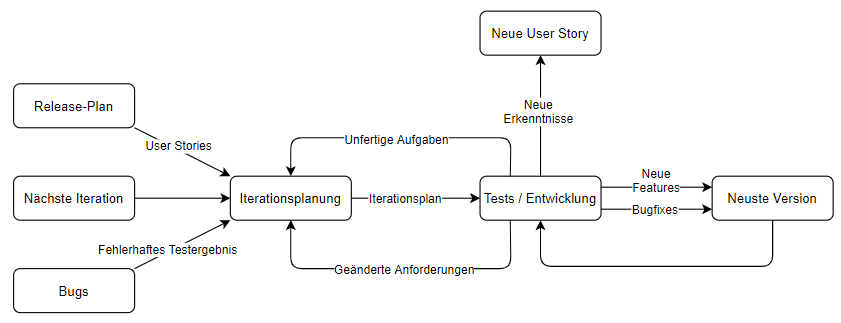
\includegraphics[width=15cm]{../images/extreme_programming.PNG}
        \caption{Ablaufdiagramm}
    \end{figure}

    \subsection{Technnologien}
    \begin{itemize}
        \item Programmiersprache: Java Version 11 mit
        \begin{itemize}
            \item JavaFX Version 15 (openjfx)
        \end{itemize}
        \item Build-Management-Tool: Gradle\cite{gradle} Version 6.7
        \item Versionskontrolle: Github Repository\cite{github} via Git\cite{git}
        \item IDE: JetBrains IntelliJ IDEA\cite{idea} 2020.2.2 (Ultimate Edition)
        \item Betriebssystem: Microsoft Windows 10 Pro 64 Bit
        \item Prozessor: Intel Core i5-3570K CPU @ 3.40GHz
        \item User Story Map: Trello Board\cite{trello}
    \end{itemize}

    \newpage

    \section{Softwarearchitektur}
    Die Gliederung der Inhalte für die Softwarearchitektur erfolgt nach der arc42-Vorlage~\cite{arc42}

    \subsection{Einführung und Ziele}
    Ziel ist die Erstellung eines Programms zur Synthetisierung von Ähnlichkeitsabbildungen einer vom Benutzer
    erstellten Verzweigungsstruktur mittels Inferieren und Optimieren von L-Systemen.
    Die wesentlichen Features des Programms sind:
    \begin{itemize}
        \item Erstellung einer Verzweigungsstruktur über eine grafische Benutzeroberfläche (\textbf{GUI})
        \item Einbindung atomarer Strukturen über externe Dateien
        \item Synthetisierung von ähnlichen Verzweigungsstrukturen anhand der erstellten Struktur
        \item Anzeigen von Verzweigungsstrukturen
    \end{itemize}
    Priorisierte (absteigend) Qualitätsziele, die bei der Erstellung des Systems umgesetzt werden sollten:
    \begin{itemize}
        \item \textbf{Funktionalität} durch Umsetzung aller Teilsysteme
        \item \textbf{Interoperabilität} durch Nutzen einer allgemeinen Repräsentation von L-Systemen, damit diese
        auch in anderen Programmen oder Algorithmen verwendet werden kann
        \item \textbf{Erweiterbarkeit} durch offene Entwurfsmuster (Design Pattern)
        \item \textbf{Modular}e Implementierung für effiziente Wartung und Erweiterung
        \item \textbf{Effizienz} durch effiziente Programmierung
        \item \textbf{Attraktivität} durch intuitive Benutzung (Benutzerfreundlichkeit)
        \item \textbf{Plattformunabhängigkeit} durch Verwenden des Java-Frameworks
    \end{itemize}

    \subsection{Kontextabgrenzung}
    \begin{figure}[H]
        \centering
        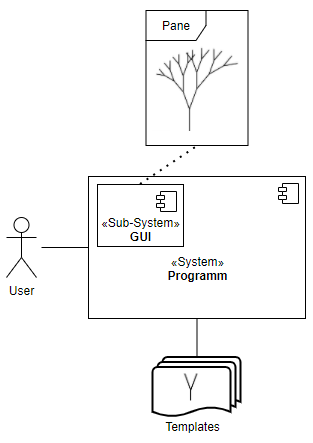
\includegraphics[width=6.2cm]{../images/Fachlicher_Kontext.PNG}
        \caption{System und Systemumgebung}
    \end{figure}
    \begin{figure}[H]
        \centering
        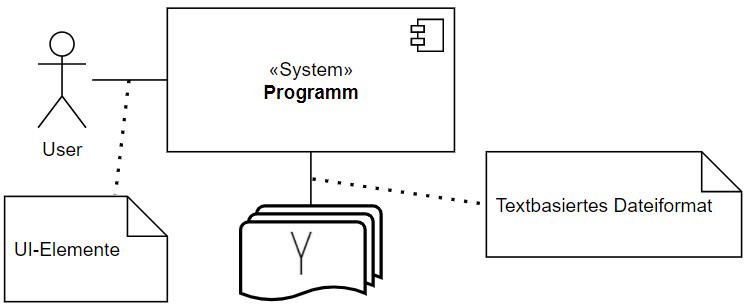
\includegraphics[width=10cm]{../images/Technischer_Kontext.PNG}
        \caption{Technische Interaktion zwischen System und Systemumgebung}
    \end{figure}

    \newpage

    \subsection{Lösungsstrategie}
    Gewählte Architekturansätze zur Erreichung der Qualitätsziele:
    \begin{center}
        \begin{tabular}{l|l}
            \textbf{Qualitätsziel} & \textbf{Architekturansatz} \\
            \hline \\
            Funktionalität &
            \begin{minipage}[t]{0.8\textwidth}
                \begin{itemize}
                    \item Grafische Benutzerschnittstelle: \textit{GUI}
                    \item Generieren der Baumstruktur: \textit{TreeGenerator}
                    \item Ableiten von L-Systemen aus Baumstrukturen: \textit{Inferer}
                    \item Generalisieren von L-Systemen: \textit{Generalizer}
                    \item Randomisieren von L-System Parametern: \textit{Randomizer}
                \end{itemize}
            \end{minipage} \\
            \\ \hline \\
            Interoperabilität &
            \begin{minipage}[t]{0.8\textwidth}
                Durch das Nutzen allgemeingültiger mathematischer Beschreibungen sollen erstellte
                L-Systeme in Fremdsystemen, wie Online Visualisierer, genutzt werden können
            \end{minipage} \\
            \\ \hline \\
            Erweiterbarkeit &
            \begin{minipage}[t]{0.8\textwidth}
                Das Nutzen des \textbf{Pipeline Design Pattern}s soll das Erweitern des Systems durch
                Hinzufügen weiterer Teilschritte (\textbf{Pipes}) erleichtern.
                Trennung der grafischen Oberfläche und der Logik durch Aufbauen des Szenengraphen über ein
                XML-Dateiformat
            \end{minipage} \\
            \\ \hline \\
            Modularität &
            \begin{minipage}[t]{0.8\textwidth}
                Sowohl eine sinnvolle Aufteilung von Funktionalitäten auf Dateien und Pakete (\textbf{Package}s), als
                auch effiziente Datenkapselung und geschlossene Informationskontexte sorgen für Modularität des
                Programms
            \end{minipage} \\
            \\ \hline
        \end{tabular}
    \end{center}

    \newpage

    Die Implementierung des Programms setzt sich aus folgenden Teilschritten zusammen:
    \begin{itemize}
        \item Erstellung der \textit{GUI} (Paket gui, tree) mit
        \begin{itemize}
            \item UI-Elementen
            \item Render-Canvas
            \item Dateianbindung der Templates
            \item Erstellung der repräsentativen Baumstruktur\\ (\textit{treeGenerator}, Paket tree)
        \end{itemize}
        \item Implementierung der Subsysteme als Pipes
        \begin{itemize}
            \item \textit{Inferer} (Paket grammar): Ableiten eines kompakten L-Systems aus einer Baumstruktur
            \item \textit{Generalizer} (Paket grammar): Generieren eines generalisierten L-Systems anhand eines
            "`kleinen"' L-Systems
            \item \textit{Randomizer} (Paket grammar): Erzeugung von L-Systemen, die der erstellen
            Verzweigungsstruktur "`ähnlich"' sind
        \end{itemize}
        \item Komponenten- und Systemtests
    \end{itemize}
    \begin{center}
        \begin{tabular}{l|l}
            \textbf{Subsystem} & \textbf{Umsetzung} \\
            \hline \\
            GUI &
            \begin{minipage}[t]{0.8\textwidth}
               JavaFX als Framework zur Erstellung von grafischen und interaktiven Inhalten.
                Erstellung der Baumstruktur über dynamisches Erzeugen von Konten während der Strukturierung der
               Verzweigungsstruktur
            \end{minipage} \\
            \\ \hline \\
            Inferer &
            \begin{minipage}[t]{0.8\textwidth}
                Algorithmus zum Iterieren maximaler Sub-Bäume und deren Reduzierung mittels Ersetzung durch Symbole
                und der zugehörigen Produktionsregel, bis eine Kostengrenze, die durch eine Kostenfunktion abgebildet
                werden kann, erreicht ist
            \end{minipage} \\
            \\ \hline \\
            Generalizer &
            \begin{minipage}[t]{0.8\textwidth}
                Algorithmus zum Erweitern eines L-Systems um nicht-deterministischer Regeln und Erkennen rekursiver
                Strukturen
            \end{minipage} \\
            \\ \hline \\
            Randomizer &
            \begin{minipage}[t]{0.8\textwidth}
    ddd         sfevdhbnreaydtydbfsdxc
            \end{minipage} \\
            \\ \hline
        \end{tabular}
    \end{center}

    \newpage

    \subsection{Bausteinsicht}
    \underline{Ebene 1}
    \begin{figure}[H]
        \centering
        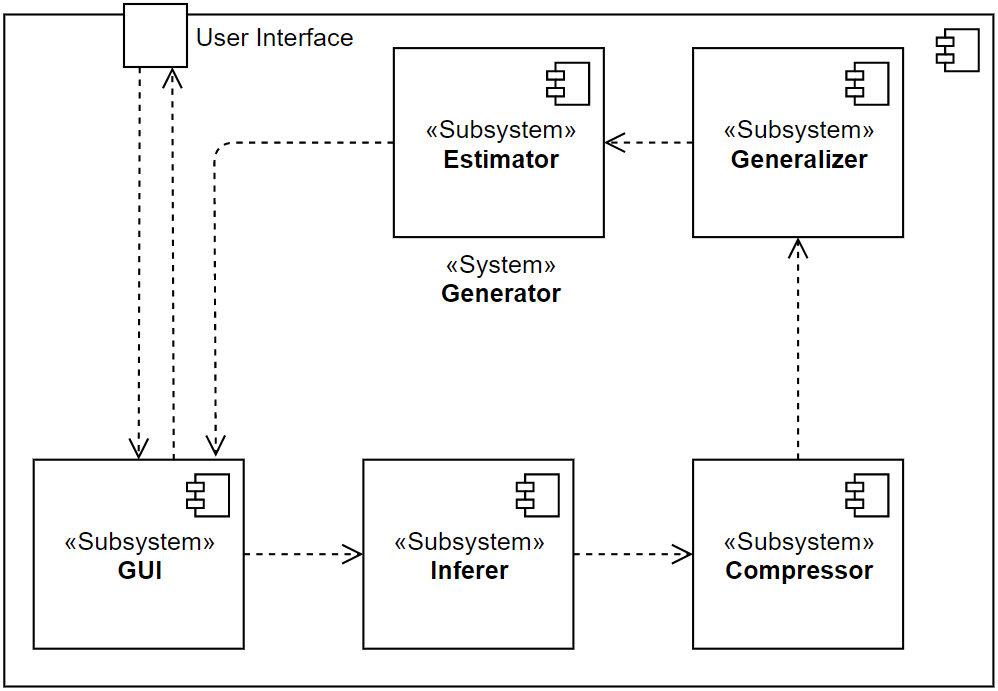
\includegraphics[width=12cm]{../images/Bausteinsicht_Ebene_1.PNG}
        \caption{Subsysteme mit fachlichen Abhängigkeiten}
    \end{figure}
    \underline{Ebene 2}
    \begin{figure}[H]
        \centering
        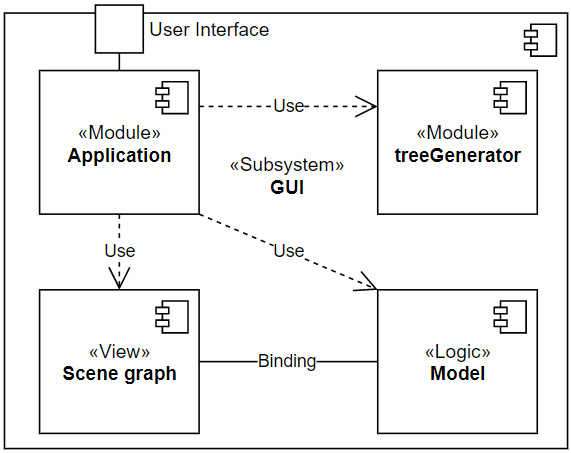
\includegraphics[width=9cm]{../images/Bausteinsicht_Ebene_2.PNG}
        \caption{Subsystem GUI}
    \end{figure}

    \subsection{Laufzeitsicht}
    \begin{figure}[H]
        \centering
        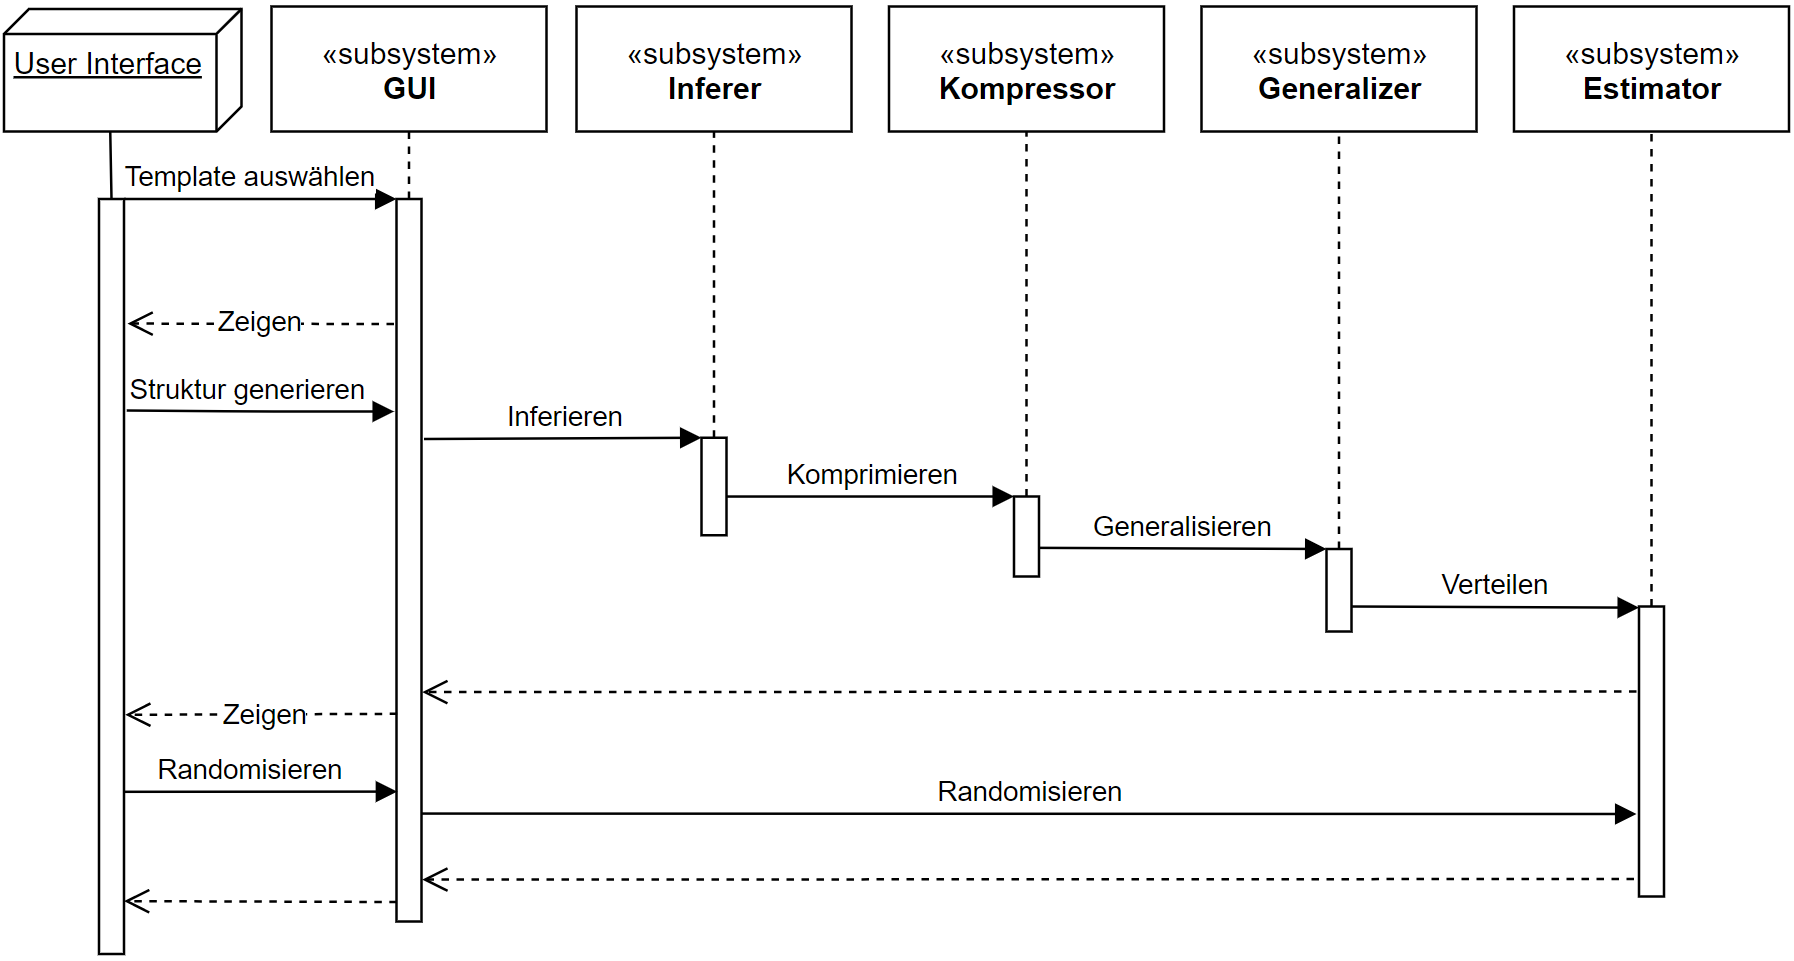
\includegraphics[width=14cm]{../images/Laufzeitsicht.PNG}
        \caption{Laufzeitsicht}
    \end{figure}

    \subsection{Verteilungsicht}
    \begin{figure}[H]
        \centering
        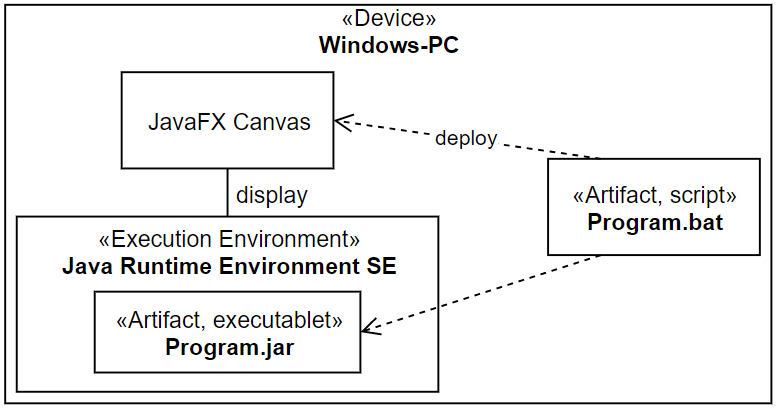
\includegraphics[width=10cm]{../images/Verteilungssicht.PNG}
        \caption{Infrastruktur Windows-PC}
    \end{figure}

    \subsection{Konzepte}

    \subsubsection{Testbarkeit}
    Um eine ausreichende Testabdeckung zu erreichen, werden Klassen als kleinstmögliche zu testende Einheit definiert
    und durch Komponententests geprüft.
    Der Name eines Tests setzt sich aus dem Präfix als Name der zu testenden Klasse oder Releases und dem Suffix
    "`Test"'
    zusammen.
    Testsubjekte werden als \textbf{Blackbox} behandelt, also anhand der Spezifikation getestet.
    Da die zugrunde liegende Java-Spezifikation JavaFX für einige Tests initialisiert werden müsste,
    werden die entsprechenden Tests nicht implementiert.
    \begin{center}
        Bsp.: Klasse \textit{Inferer} mit Komponententest \textit{InfererTest}
    \end{center}
    Da jedes Release der Implementierung ein funktionsfähiges System beinhaltet, kann auf Integrationstests
    verzichtet werden.
    Weiter wird ein Release anhand von funktionalen und nicht-funktionalen Anforderungen getestet.
    Anhand dieser Systemtests wird geprüft, ob Gesamtspezifikationen umgesetzt worden sind.
    \begin{center}
        Bsp.: Release 2 mit Systemtest \textit{Release2Test}
    \end{center}
    Zum Schluss der Implementierung wird ein Akzeptanztest durchgeführt.

    \subsubsection{Validierung}
    Der Benutzer des Systems nutzt ein grafische Schnittstelle.
    Somit kann sichergestellt werden, dass dieser keine ungültigen Eingaben tätigt.
    Werden Template-Dateien unter einem bestimmten Dateipfad nicht gefunden, wird eine \textit{NotFound}-Exception
    protokolliert und dem Benutzer eine Nachricht über ein Pop-up mitgeteilt.
    Eine \textit{IllegalArgumentException} wird verzeichnet und ausgegeben, wenn eingelesene Template-Dateien
    strukturelle Fehler aufweisen.

    \subsubsection{Fehlerbehandlung}
    Zur Fehlersuche und -behandlung biete sich eine Protokollierung über Vorgänge, Fehler und Ausnahmen an.
    Bestimmte Fehler werden dem Benutzer weitergegeben und grafisch angezeigt.
    Folgende Subsysteme werden in das Programm integriert:
    \begin{itemize}
        \item Ausnahmebehandlung (Exception Handling) und
        \item Protokollierung (Logging)
    \end{itemize}
    Erwartete Exceptions werden jeweils mit eigenen Klassen abgebildet, die von einer entsprechenden Klasse aus der
    Exception-Hierarchie abgeleitet sind.
    Das Logging ist statisch und überall im System zugreifbar, um eine einheitliche Protokollierung zu gewährleisten.

    \subsubsection{Datenstrukturen}
    TODO: Klassendiagramm aus IntelliJ generieren

    \subsubsection{Workflows \& Algorithmen}
    Um als Benutzer des Systems eine Verzweigungsstruktur zu erstellen, wird folgender Arbeitsablauf umgesetzt:
    \begin{algorithm}[caption={Erstellen einer Verzweigungsstruktur}, label={alg1}]
Erster Anker ist vorselektiert
Wiederhole, bis Struktur fertiggestellt ist:
    Selektiere ein Template aus der Liste
    Setzt Parameter
    Bestätige Auswahl und Parameter
    Zeichne ausgewähltes Template mit Parametern
    Wähle nächsten Anker aus
    \end{algorithm}
    \\~\\~\\
    Aus der Verzweigungsstruktur kann nun ein L-System erzeugt werden:
    \\~\\
    Für $\mathcal{L}=\langle M,\omega,R \rangle$:
    \begin{algorithm}[caption={Inferieren eines L-Systems aus einer Baumstruktur}, label={alg2}]
Initialisierung:
    $M=\{F,S\}$
    $\omega=S$
    $R \gets \{\alpha$: $S \rightarrow A\}$
    $\beta=$ nächster Knoten*
    $M \gets \gamma \in \{A,B,\dots,Z\}$, mit $\gamma \notin M$

Schleife:
    $\delta=$ Wort von $\beta$
    $\forall \{X,Y,Z\} \in \delta:$
        Ersetze mit $\zeta \in \{A,B,\dots,Z\}$, mit $\zeta \notin M$
        $M \gets \zeta$
    $R \gets \{\gamma\rightarrow\delta\}$
    Wenn es ein Symbol $\eta$ in $M\setminus\{F,S\}$ gibt mit $\{\eta \rightarrow bel.\} \notin R$:
        $\gamma=\eta$
    Sonst:
        Breche Schleife ab
    $\beta=$ nächster Knoten*
    \end{algorithm}
    \blfootnote{* nach Breitensuche, beginnend bei Wurzelknoten S}

    \newpage

    Um ein kompakteres, gewichtetes L-System zu erzeugen, werden sich wiederholende Unterrbäume gesucht und ersetzt.
    Die Gewichtung wird angewendet, um das erzeugte L-System in ein System mit kleiner Regelmenge ($w_l=1$) oder mit
    großer Regelmenge ($w_l=0$) umzuwandeln:
    \begin{algorithm}[caption={Erstellen eines kompakten L-Systems mit Gewichtung $w_l$}, label={alg3}]
Initialisierung:
    $\mathcal{L}^+ \leftarrow L_s$*
    $\mathcal{L}=\emptyset$
    Setze Gewichtungsparameter $w_l \in [0,1]$
    Finde maximalen Unterbaum $T'$ aus $T$** mit Wiederholungen $n$

Reduzierung:
if n > 1
    Ersetze alle Vorkommen von $T'$ mit dem selben Symbol $\gamma \in \{A,B,\dots,Z\}$
    $R \leftarrow \{\gamma \rightarrow L_s\}$ mit $L_s$ aus $T'$, $R$ aus $\mathcal{L}$
    if $C_i(\mathcal{L}) \geq C_i(\mathcal{L}^+)$
        break
    $T \leftarrow T'$
    $\mathcal{L}^+ \leftarrow \mathcal{L}$
    Finde maximalen Unterbaum $T'$ aus $T$ mit Wiederholungen $n$
    \end{algorithm}
    \blfootnote{* $L_s$ als Zeichenkette des Ausgeführten L-Systems $\mathcal{L}=\langle M,\omega,R \rangle$}
    \blfootnote{** $T$ als Baumstruktur des L-Systems}

    Die Kostenfunktion stellt die Anzahl Symbole aller \textit{RHS} der Produktionsregeln mit der Menge an
    Anwendungen der \textit{LHS} gegenüber:
    \begin{algorithm}[caption={Kostenfunktion $C_i$ mit Gewichtung $w_l$}, label={alg4}]
$C_i(\mathcal{L})= \sum\limits_{A(P) \rightarrow M^* \in \mathcal{L}} w_l * |M^*| + (1 - w_l) * N(A(P)\rightarrow
M^*)$***
    \end{algorithm}
    \blfootnote{*** $N(\cdot)$ als Zählfunktion für die Anzahl Wiederholungen einer \textit{LHS} einer Regel in einem
    ausgeführten L-System}

    Da das kompakte L-System eine Repräsentation der vom Benutzer erzeugten Verzweigungsstruktur darstellt, werden
    nun ähnliche Regeln miteinander verbunden und mit einer Wahrscheinlichkeit versehen, um nicht-deterministische
    Regeln hinzuzufügen.

    \begin{algorithm}[caption={Längenfunktion $L$ für Grammatiken}, label={alg5}]
$L(\mathcal{L}) = |M| + \sum\limits_{A(P) \rightarrow M^* \in \mathcal{L}} |M^*|$
    \end{algorithm}

    \begin{algorithm}[caption={Kostenfunktion $C_g$ mit Gewichtung $w_0$}, label={alg6}]
$C_g(\mathcal{L}^*, \mathcal{L}^+) = w_0 * (L(\mathcal{L}^*) - L(\mathcal{L}^+)) + (1 - w_0) + D_g
(\mathcal{L}^+, \mathcal{L}^*)$
    \end{algorithm}

    \begin{algorithm}[caption={Generalisieren eines L-Systems mit Gewichtung $w_0$}, label={alg7}]
Initialisierung:
    Regelpaar $p* = \emptyset$
    $\mathcal{L}^* = \mathcal{L}^+$
    $C_g^{old} = C_g(\mathcal{L}^* + \{p^*\}, \mathcal{L}^*)$

Schleife:
do
    Finde Regelpaar $p^*$ mit minimalen Kosten $C_g(\mathcal{L}^* + \{p_i\}, \mathcal{L}^*), \forall p_i \in
\mathcal{P}$*
    if $C_g(\mathcal{L}^* + \{p^*\}, \mathcal{L}^*) \geq 0$
        break
    $c^* = C_g(\mathcal{L}^* + \{p^*\}, \mathcal{L}^*) - C_g^{old}$
    $C_g^{old} = C_g(\mathcal{L}^* + \{p^*\}, \mathcal{L}^*)$
    $\mathcal{L}^* = \mathcal{L}^* + \{p^*\}$
while $c^* \leq 0$
    \end{algorithm}
    \blfootnote{* $\mathcal{P}$ als Menge aller möglichen Regelpaaren aus $\mathcal{L}^*$}


    \subsubsection{Entscheidungen}
        \underline{Mutable or Immutable Objects?}\\~\\
        \underline{Risiken}\\~\\
        \underline{Qualitätsmerkmale}\\~\\
        \underline{Alternativen}\\~\\
        \underline{Aufwand der Implementierung}

    \newpage

    ~\nocite{*}
    \renewcommand{\refname}{Quellen}
    \bibliography{konzepte}
    \bibliographystyle{plain}
    \addcontentsline{toc}{section}{Quellen}

\end{document}